\documentclass[tikz,border=10pt]{standalone}
\usepackage{amsmath}
\begin{document}
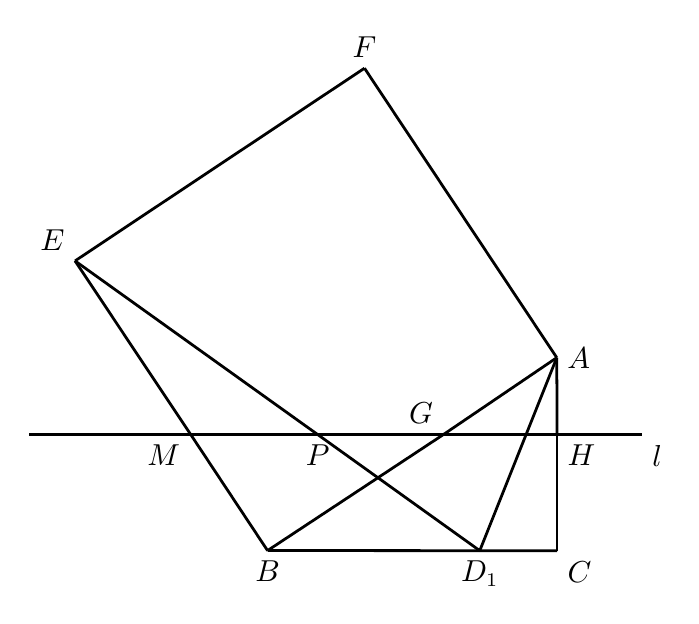
\begin{tikzpicture}[line join=round, line width=1.0pt,
  lbl/.style={font=\fontsize{10.5}{12.6}\selectfont}]
\coordinate (A) at (2.663,-0.577);
\coordinate (B) at (-1.010,-3.027);
\coordinate (C) at (2.667,-3.029);
\coordinate (F) at (0.221,3.099);
\coordinate (G) at (1.224,-1.553);
\coordinate (H) at (2.667,-1.553);
\coordinate (M) at (-1.986,-1.553);
\coordinate (P) at (-0.374,-1.553);
\coordinate (GeoTailH) at (3.741,-1.553);
\coordinate (GeoTailP) at (1.670,-3.016);
\coordinate (GeoTailG) at (1.991,-1.030);
\coordinate (GeoTailM) at (-4.039,-1.553);



\coordinate (E) at (-3.455,0.652);
\coordinate (D1) at (1.685,-3.028);


\draw (E)--(F);
\draw (F)--(A);
\draw (A)--(H);
\draw (H)--(C);
\draw (C)--(D1);
\draw (D1)--(B);
\draw (B)--(M);
\draw (M)--(E);
\draw (A)--(G);
\draw (G)--(B);


\draw (E)--(P);
\draw (P)--(D1);


\draw (A)--(D1);


\draw (GeoTailM)--(M);
\draw (M)--(P);
\draw (P)--(G);
\draw (G)--(H);
\draw (H)--(GeoTailH);


\node[above left,lbl] at (E) {$E$};
\node[above,lbl] at (F) {$F$};
\node[right,lbl] at (A) {$A$};
\node[below,lbl] at (B) {$B$};
\node[below right,lbl] at (C) {$C$};
\node[below,lbl] at (D1) {$D_1$};
\node[above left,lbl] at (G) {$G$};
\node[below left,lbl] at (M) {$M$};
\node[below,lbl] at (P) {$P$};
\node[below right,lbl] at (H) {$H$};
\node[below right,lbl] at (GeoTailH) {$l$};
\end{tikzpicture}
\end{document}